\documentclass{article} 
\usepackage{graphicx}
\title{Bailando Differentiator} 
\author{Dmit} 
\date{December 2023} 
\begin{document} 
\maketitle 
\section{Bailando-Differentiating Func} 
Si senor efectos especiales ye ye ye: $ln(x)$  \newline Si senor una tentacion ye ye ye: $x$ Tu y yo a la fiesta: $1$  \newline Tu y yo toda la noche: $\frac{1}{x}*1$  \newline \newline Optimization bailnado: \newline Tu y yo a la fiesta: $\frac{1}{x}$  \newline Tu y yo: $\frac{1}{x}$  \newline \begin{figure}
\centering
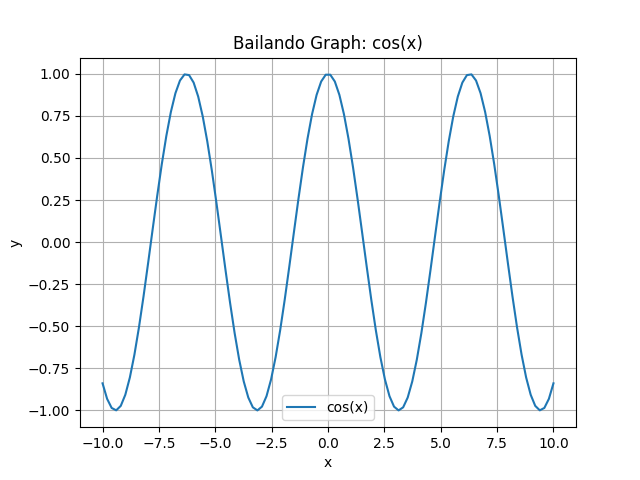
\includegraphics[width=0.8\linewidth]{Bailando Graph.png}
\caption{Bailando: Graph}
\label{fig:my_image}
\end{figure}
 \newline \newline Optimization bailnado: \newline Bailando bailando amigos adios: $\frac{1}{x}$  \newline 
\end{document}